\begin{wrapfigure}{r}{80mm}
\vspace*{-4mm}
\centerline{
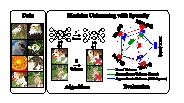
\includegraphics[width=80mm,height=!]{figs/overview_new.pdf}
}
% \hspace*{-2mm}
\vspace*{-2mm}
\caption{\footnotesize{
Schematic overview of our proposal on model sparsity-driven {\MU}. Evaluation at-a-glance shows the performance of three unlearning methods (retraining-based exact unlearning, finetuning-based approximate unlearning \cite{golatkar2020eternal}, 
and proposed   unlearning on 95\%-sparse model) under five metrics:  
unlearning accuracy ({\UA}), membership inference attack (MIA)-based unlearning efficacy, accuracy on remaining data ({\RA}), testing accuracy (\TA), and run-time efficiency (\RTE); see summary in \textbf{Tab.\,\ref{tab: summary_MU_methods_metrics}}.
The unlearning scenario is given by class-wise forgetting, where data points of a single class are scrubbed.  Each metric is normalized to $[0,1]$ based on the best result across unlearning methods 
  for ease of visualization.
  %, while the actual best value  is provided.
%Each performance metric is normalized to $[0,1]$ based on the best result  across unlearning methods.
%We normalized each metric by dividing the best performance in that metric, and $100\%$ denotes the best performance on each metric. 
Results indicate that \textcolor{blue}{model sparsity} reduces the gap between \textcolor{red}{exact} and \textcolor{ForestGreen}{approximate} {\MU} without loss in efficiency. 
%\JC{[updated]}
% \SL{change to 95\%-sparse case.}
% \JC{Add l1-sparse unlearn?} \SL{[Yes. You can use $\ell_1$ to replace `95\% sparse finetuning'.]}
% \SL{talk to me about this figure.}
%\JC{An overview of our method (briefly describe the figure) ... The radar chart on the right gathered the evaluation metrics at a glance. (Describe all metrics, especially MIA)} 
%\SL{[@Yuguang, @Jiancheng, @Jinghan. Talk to me.]} 
%\YL{annotating the five metrics in the captions would be helpful..}
%\PS{How come dense model unlearning is not a pentagon in the radar chart? Or is it hidden behind sparsity aware pentagon?}
}}
\label{fig: results_highlights}
%\end{wrapfigure}
%\end{figure}
\vspace{-7.1mm}
\end{wrapfigure}
%\vspace*{-8mm}
% \begin{figure}[htb]
% %\begin{wrapfigure}{r}{80mm}
% %\vspace*{-6mm}
% \centerline{
% %\begin{tabular}{cc}
% %\hspace*{0mm}\includegraphics[width=.3\textwidth,height=!]{figure/performance_comparison.pdf}  
% %&
% %\hspace*{-4mm}
% 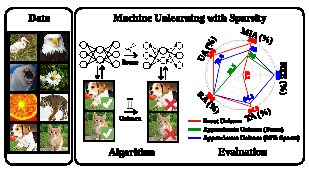
\includegraphics[width=.49\textwidth,height=!]{figs/Overview.pdf}
% % \\
% % \hspace*{2mm}\footnotesize{(a) Test accuracy vs. pruning ratio.} &   \footnotesize{(b) Runtime of pruning.}
% %\end{tabular}
% }
% \vspace*{-3mm}
% \caption{\footnotesize{
% %\JC{"95\% Sparse" -> "Sparse" in the figure}
% Schematic overview of our proposal on model sparsity-driven {\MU}. Performance at-a-glance is provided when evaluating three unlearning methods (retraining-based exact unlearning, finetuning-based approximate unlearning \cite{golatkar2020eternal}, 
% and proposed finetuning-based  unlearning on 95\%-sparse model) under five   metrics,  
% unlearning accuracy ({\UA}), membership inference attack (MIA)-based unlearning efficacy, accuracy on remaining data ({\RA}), testing accuracy (\TA), and run-time efficiency (\RTE), as will be shown in Table\,\ref{tab: summary_MU_methods_metrics}. Results show that \textcolor{blue}{model sparsity} reduces the gap between \textcolor{red}{exact} and \textcolor{ForestGreen}{approximate} {\MU}.
% %\JC{An overview of our method (briefly describe the figure) ... The radar chart on the right gathered the evaluation metrics at a glance. (Describe all metrics, especially MIA)} 
% %\SL{[@Yuguang, @Jiancheng, @Jinghan. Talk to me.]} 
% %\YL{annotating the five metrics in the captions would be helpful..}
% %\PS{How come dense model unlearning is not a pentagon in the radar chart? Or is it hidden behind sparsity aware pentagon?}
% }}
% \label{fig: results_highlights}
% %  \vspace*{-3.8mm}
% %\end{wrapfigure}
% %\end{figure}
% \end{figure}
